%%%%%%%%%%%%%%%%%%%%%%%%%%%%%%%%%%%%%%%%%%%%%%%%%%%%%%%%%%%%%%%%%%%%%%%%%%%%%%
%
% Main content starts here
%
%%%%%%%%%%%%%%%%%%%%%%%%%%%%%%%%%%%%%%%%%%%%%%%%%%%%%%%%%%%%%%%%%%%%%%%%%%%%%%


\chapter{Introduction}
\label{sec:introduction}

This is a typical human-computer interaction thesis structure for an introduction which is structured in four paragraphs as follows:
% First Paragraph
% CORE MESSAGE OF THIS PARAGRAPH:
\todo{P1.1. What is the large scope of the problem?}
\todo{P1.2. What is the specific problem?}

% Second Paragraph
% CORE MESSAGE OF THIS PARAGRAPH:
\todo{P2.1. The second paragraph should be about what have others been doing}
\todo{P2.2. Why is the problem important? Why was this work carried out?}

% Third Paragraph
% CORE MESSAGE OF THIS PARAGRAPH:
\todo{P3.1. What have you done?}
\todo{P3.2. What is new about your work?}

% Fourth paragraph
% CORE MESSAGE OF THIS PARAGRAPH:
\todo{P4.1. What did you find out? What are the concrete results?}
\todo{P4.2. What are the implications? What does this mean for the bigger picture?}

LaTeX hints are provided in \autoref{chap:latexhints}.

\chapter{Background and related Work}
\section{Relevante Konzepte und Definitionen}
\subsection{Deepfakes}
"Deepfakes - Wenn man Augen und Ohren nicht mehr trauen kann" \cite{bildungDeepfakesWennMan2023} - 
So steigt Journalist und Autor der Bundeszentrale für politische Bildung Tim Walter in seinem Artikel über die Gefahren von Deepfakes ein. 
Dies ist nur eins von vielen Beispielen (Weitere Beispiele im Fußbereich) das zeigt, 
dass Deepfakes mittlerweile ein ernstgenommenes Thema in der nicht-technischen Medienwelt und Gesellschaft sind. 
Doch was genau sind eigentlich Deepfakes? 

\textcite{gambinDeepfakesCurrentFuture2024} beschreiben das Konzept Deepfake als "generation of fake digital content or manipulated of genuine one through the use of DL techniques." \cite[S. ?]{gambinDeepfakesCurrentFuture2024},
also frei übersetzt als die Erzeugung von gefälschten digitalen Inhalten oder die Manipulation echter Inhalte durch den Einsatz von Deep Learning Techniken. 
Deep Learning ist ein Teilgebiet der Künstlichen Intelligenz, genauer gesagt des Machine Learning, in dem es darum geht, mithilfe einer Reihe von Methoden automatisch Muster in Daten zu erkennen und diese zur Vorhersage zukünftiger Daten oder Entscheidungen zu verwenden \autocite[S. 1]{murphyMachineLearningProbabilistic2012} . 
Weiter schreiben Gambin et. al "The content inlcudes video, image, audio, and text among other sources." 
In einer ähnlichen Definition heißt es, dass bei Deepfake Videos in den meisten Fällen in einem schon existierenden Video das Abbild einer Person über den Körper einer anderen Person gelegt wird. 
Dadurch sieht es aus, als würde die Person dessen Abbild darüber gelegt wurde die Aktivitäten der anderen Person ausführen \autocite{harrisVideoDemandWhat2021}.
Währenddessen teilen \textcite{juefei-xuCounteringMaliciousDeepFakes2022} Deepfakes in die vier Kategorien "(i) entire face synthesis, (ii) attribute manipulation, (iii) identity swap, and (iv) expression swap (i.e., reenactment)". 
Schon an diesen Beispielen lässt sich erkennen, dass Deepfakes in unterschiedlichen Formen vorkommen.

Nachdem nun geklärt ist, was Deepfakes eigentlich sind, fehlt noch wo Deepfakes ihren Ursprung \cite{AIAssistedFakePorn2017} haben. 
Dazu schreiben \textcite{kernerPornDiscreditationEpistemic2021} "Deepfakes got started in 2017 [...] when an eponymous Reddit user enlisted open-source software from Google and elsewhere to apply scattered academic research to face-swapping". 
Die erste mediale Berichterstattung folgte im Dezember 2017 durch den Artikel \textcite{AIAssistedFakePorn2017} im Vice Tech Magazin Motherboard von Samantha Cole.
Seitdem nimmt die Verbreitung von Deepfakes immer weiter zu, was man unter anderem bei \textcite{ranaDeepfakeDetectionSystematic2022,westerlundEmergenceDeepfakeTechnology2019,gamagePDFEmergenceDeepfakes} sieht. 
Auch die Google Suchtrends zum Keyword "Deepfake" bestätigen diese Aussage, siehe Grafik \ref{fig:suchtrend-grafik}.
\begin{figure} [htbp]
    \centering
    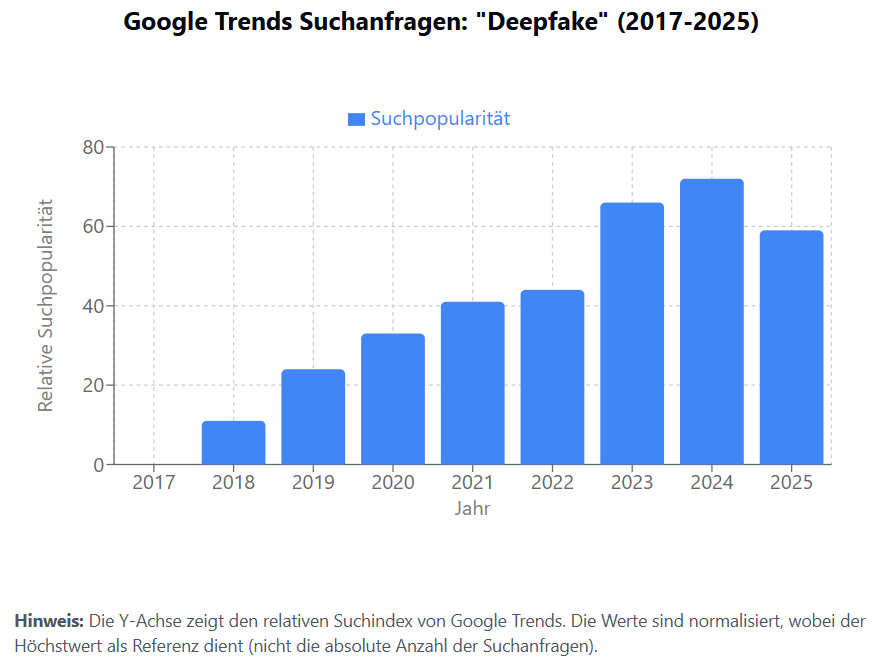
\includegraphics[width=0.8\textwidth]{GrafikGoogleTrendDeepfake.png}
    \caption{Google Suchtrend zum Keyword "Deepfake"}
    \label{fig:suchtrend-grafik}
\end{figure}

Seitdem werden Deepfakes allerdings auch immer wieder für negative Zwecke eingesetzt. 
Ein großer Einsatzbereich und auch der Ursprung von Deepfakes ist die Pornographie \autocite{ajderDeeptraceLabReport}. 
Aber auch abseits von Pornographie gibt es noch mehr kriminelle oder bösartige Einsatzbereiche von Deepfakes. 
Darunter sind unter anderem "spreading misinformation, creating political instability, or various cybercrimes" \cite{ranaDeepfakeDetectionSystematic2022} 
oder wie \textcite{gambinDeepfakesCurrentFuture2024} die Konsequenzen von Deepfakes als "far reaching, including the potential to ignite political or religous tensions between nations, decieve the public, disrupt financial markets, perpetrate acts of sabotage, fraud, scams, obstruct justice, and much more" beschreiben.
Im Folgenden einige Beispiele aus der Praxis von Fällen in denen Deepfakes mit krimineller oder bösartiger Absicht eingesetzt wurden.
\begin{itemize}
    \item Manipulation in der Politik: Ein Audio-Deepfake in dem der slowakische Spitzenkandidat Michal Šimečka scheinbar mit einer 
        Journalistin über das Kaufen von Wählerstimmen diskutiert, wird kurz vor der Parlamentswahl im Oktober 2023 veröffentlicht. 
        Dieser Deepfake wurde strategisch kurz vor der Wahl platziert und durch die slowakische Regelung, 
        dass 48 Stunden vor der Wahl in den Medien kein Wahlkampf mehr betrieben werden darf, wurde eine Richtigstellung noch erschwert. \autocite{pawelecPolitischeManipulationUnd2024}
    \item Revenge Porn und andere nicht-einvernehmliche Inhalte: 
        Im Fall von Hannah Grundy wurden Deepfake Fotos mit pornographischen Inhalten von ihr auf einer Website "The destruction of Hannah" hochgeladen \autocite{WomansDeepfakeBetrayal2025}.
        In einem anderen Fall wurde im türkischen Wahlkampf ein Deepfake Video mit pornographischem Inhalt von Kandidat Muharrem İnce veröffentlicht, 
        was dessen Rücktritt aus dem Wahlkampf zur Konsequenz hatte. \autocite{TurkishPresidentialCandidate2023}
    \item Verleumdung von bekannten Persönlichkeiten: Prominente Personen werden regelmäßig Opfer von Deepfakes, 
        die ihren Ruf schädigen sollen oder Produkte in ihrem Namen ohne ihre Zustimmung bewerben \autocite{PDFImpactDeepfake2025}.
    \item Manipulierte Unternehmenskommunikation: Durch gezielte Deepfakes können Angestellte oder Aktionäre getäuscht und betrogen werden \autocite{PDFImpactDeepfake2025}.
\end{itemize}
Bei all den negativen Beispielen ist zu beachten, dass die Deepfake Technologie an sich neutral ist und auch vielfache Weise positiv eingesetzt werden kann. Im Folgenden einige positive Beispiele wie Deepfakes eingesetzt werden können \autocite{westerlundEmergenceDeepfakeTechnology2019}:
\begin{itemize}
    \item Filmindustrie: Das Erzeugen der Stimmen von Schauspielern die ihre Stimme wegen einer Krankheit verloren haben. 
        In einem anderen Fall hat 2019 eine Malaria Kampagne David Beckham durch Deepfake Technologie multilingual wirken lassen um möglichst viele Menschen ansprechen zu können.
    \item Medizinischer Bereich: Durch Deepfakes können Alzheimer Patienten mit jüngeren Gesichtern interagieren, die sie möglicherweise wiedererkennen. 
    \item Wirtschaftsbereich: Das digitale Anprobieren von Kleidung kann durch Deepfake Technologie ermöglicht werden.
\end{itemize}
Diese Beispiele zeigen, dass die Deepfake Technologie jetzt schon in der Gesellschaft verankert ist, und sich in Zukunft noch weiter ausbreiten wird.

\subsection{Public Displays}
In Krankenhäusern, Universitäten, Bahnhöfen oder Shopping Center. 
An immer mehr öffentlichen oder halb-öffentlichen Orten findet man mittlerweile interaktive Bildschirme, 
nachfolgend auch "Public Displays" genannt. Nach \textcite{parkerDoesPublicStill2018} ist ein Public Display 
ein "medium that brings digital content into the real world and into the eyes of the general public." \cite{parkerDoesPublicStill2018} 
Waren es früher noch nur große Bildschirme die Werbung, Videos oder andere Informationen ohne Möglichkeit zur Interaktion angezeigt haben \cite{PDFEnticingPeople}, 
werden diese heute immer mehr eingesetzt um Informationen visuell und vor allem oft interaktiv darzustellen \cite{hinrichsInteractivePublicDisplays2013}. 
Beispiele aus eigener aktueller (Mai 2025) Erfahrung von Public Displays sind die interaktiven Bildschirme im Münchner Olympia-Einkaufszentrum, 
mit deren Hilfe Besucher Informationen über die verschiedenen Läden einholen können. 
Ein weiteres Beispiel sind Public Displays in Hauseingängen von Mehrparteienhäusern, 
die von den Hausbewohnern zum Informationsaustausch genutzt werden, aber auch um Informationen von der Hausverwaltung an die Bewohner weitergeben zu können.
Einen Schritt weiter geht die Forschung zu sogenannten "public security user interfaces". 
Diese sind definiert als "any type of interface positioned in shared, 
non-personal areas that offers information or the opportunity to interact with security-related topics" \cite{murtezajPublicSecurityUser2025}. 
Durch die zunehmende Bedrohung von Cyber Angriffen ist die Idee entstanden, mithilfe von Public Displays die öffentliche Wahrnehmung von Sicherheitsthemen zu erhöhen. 
Eingesetzt werden diese Interfaces, um bestimmte Ziele zu erreichen, die im folgenden kurz vorgestellt werden.
\begin{itemize}
    \item Creating Awareness: Das Ziel ist, die Nutzer auf mögliche Sicherheitsrisiken aufmerksam zu machen, wie z.B. die Verwendung desselben Passworts für verschiedene Plattformen.
    \item Triggering Actions: Der Nutzer soll dazu gebracht werden, direkt eine Aufgabe in Bezug auf einen Sicherheitsaspekt anzugehen. 
        Ein Beispiel wäre, den Nutzer aufzufordern, verfügbare Sicherheitsupdates für sein Gerät zu installieren.
    \item Sparking Conversation: Hier ist das Ziel, durch das Public security user interface eine Diskussion über bestimmte Sicherheitsthemen anzustoßen, 
        beispielsweise durch fun facts oder andere gesprächsanregende Informationen. 
        Dadurch soll das Thema der Cyber Security noch mehr in den Alltag integriert werden.
\end{itemize}
Diese Ziele geben jetzt schon zahlreiche Einsatzmöglichkeiten und lassen Raum für weitere \cite{murtezajPublicSecurityUser2025}.

\section{Existing technologies}
\subsection{Creation of deepfake technology}
Nachdem nun bekannt ist, was Deepfakes eigentlich sind und wo diese ihren Ursprung haben, wollen wir nun klären wie diese erzeugt werden.
Die ersten Deepfake Videos wurden wie schon beschrieben 2017 von einem anonymen Reddit User erstellt, 
der mit verschiedenen Open-Source Programmen frühe face-swapping Algorithmen aus der Forschung angewandt hat \cite{kernerPornDiscreditationEpistemic2021}. 
Ausführlicher beschreibt es nur \textcite{AIAssistedFakePorn2017} in ihrem Artikel für das Vice Tech Magazin Motherboard. 
Demnach hat der Reddit User "deepfakes" mithilfe von verschiedenen Open-Source Bibliotheken wie Keras und Trainingsbildern aus Google Bilder, 
Stock Fotos und Youtube Videos einen Algorithmus trainiert, der dann in die entsprechenden Vorlagen Videos die Gesichter der Prominenten Personen einfügt \cite{AIAssistedFakePorn2017}.
Eine Technologie mit großen Fortschritten in der Erzeugung von Deepfake Inhalten ist das Modell der sogenannten "generative adversarial networks", 
eingeführt durch \textcite{goodfellowGenerativeAdversarialNetworks2014}, nachfolgend auch GANs genannt. 
Diese GANs bestehen aus zwei neuronalen Netzwerken, dem Generator und dem Discriminator. 
Diese zwei Teile werden gleichzeitig trainiert, wobei der Generator das Ziel hat, den Discriminator mit möglichst echt wirkenden Bildern zu täuschen, 
und der Discriminator das Ziel hat, sich nicht von dem Generator täuschen zu lassen \cite{benaissaOverviewGANDeepFakesDetection2024}. 
Weiterhin gibt es mittlerweile eine Menge von verschiedenen GAN Modellen die zur Erzeugung von Deepfakes genutzt werden. 
Eine Auswahl davon stellt \textcite{benaissaOverviewGANDeepFakesDetection2024}vor, darunter sind DCGAN, CycleGAN, PGGAN und einige mehr.

Im Bereich der Bilderzeugung ist mittlerweile das Modell der Diffusion Modells zum Standard geworden \cite{guptaPhotorealisticVideoGeneration} 
und hat die vorher beschriebenen GANs übertroffen \cite{williampeeblesScalableDiffusionModels}. 
Ein Model zur vollständig künstlichen Erzeugung von Deepfakes, welches zum Zeitpunkt des Schreibens für einige Schlagzeilen \cite{proschofskyGooglesNeueVideoKI2025} gesorgt hat, 
ist das video generation Model Veo 3 von Googles Deepmind. Dieses verwendet ein latent diffusion model (veo 3 tech report). 
Ein Diffusion Model lernt Bilder zu erstellen, indem es aus einem Bildrauschen schrittweise das Rauschen immer weiter entfernt \cite{guptaPhotorealisticVideoGeneration}. 
Dieses wird außerdem in einem latent space angewendet. Statt direkt auf den Pixeln zu arbeiten, 
lässt man das Model in einem "lower-dimensional latent space" \cite{guptaPhotorealisticVideoGeneration} arbeiten, was den Rechenaufwand deutlich reduziert. 
Hierfür lässt man einen Autoencoder Bilder in kleinere räumliche Repräsentationen komprimieren und das diffusion model auf diesen räumlichen Repräsentationen trainieren. 
Einige Beispiele zu was Veo 3 fähig ist, sieht man auf Googles Deepmind Youtube Channel \cite{Veo3Our}.

\subsection{technical countermeasures against deepfake technology}
Je besser das Erzeugen von Deepfakes wird, desto schwieriger werden auch die Gegenmaßnahmen zu Deepfakes. 
Hierzu gibt es auf der technischen Seite unterschiedliche Herangehensweisen, welche in aktive und passive Maßnahmen eingeteilt werden können, 
wobei sich diese generell noch in frühen Stadien befinden \cite{abbasUnmaskingDeepfakesSystematic2024}.
\subsubsection{automated detection methods}
Die passive Herangehensweise ist das klassische Erkennen von deepfakes durch Technologien die selbst auf machine learning oder sogar deep learning basieren. 
Das Literature Review von Abbas und Taeihagh zeigt hier eine Vielzahl von deep learning Technologien, 
darunter eine Menge Varianten die auf CNNs basieren, aber auch eine einige Varianten die auf den oben vorgestellten GANs basieren. 
\textcite{benaissaOverviewGANDeepFakesDetection2024} zeigen noch zwei weitere interessante Ansätze speziell für die Erkennung von deepfake Videos. 
Der eine ist die "biological signal analysis". Bei diesem werden physiologische Signale wie Blinzeln, Augenbewegung oder Herzschlag analysiert und damit die Videos auf Echtheit überprüft. 
In einem Fall wurde dafür eine Kombination aus einem convolutional neural network und einem recursive neural network verwendet, 
ein einem anderen Fall wurden auch wieder die oben genannten GANs verwendet.
Der andere Ansatz ist die "spatial and temporal features analysis". Bei diesem wird nicht wie bei den meisten anderen Ansätzen mit einzelnen Video Frames gearbeitet. 
Hier werden zeitliche und räumliche Merkmale über den Verlauf des Videos mit verschiedenen Modellen wie GANs oder CNNs analysiert und damit auf Echtheit geprüft \cite{benaissaOverviewGANDeepFakesDetection2024}.
\subsubsection{authentification systems}
Um aktiv gegen Deepfakes vorzugehen, bietet sich die Authentifizierung von echten Videos an, 
ein sogenanntes "Proof of Authenticity System" \cite{gambinDeepfakesCurrentFuture2024}. 
Hier konzentriert sich die Forschung vor allem auf blockchain basierte Technologien um echte Videos zu verifizieren. 
Diese funktionieren durch ein dezentrales Transaktionssystem, 
welches durch seine Eigenschaften nahezu fälschungssicher ist und Transaktionen allgemein sicherer und transparenter macht \cite{gambinDeepfakesCurrentFuture2024}. 
Die Idee dahinter ist, Inhalte und im speziellen Videos und Bilder bis zu ihrem Ersteller zurückverfolgen zu können, 
mitsamt wichtigen Metadaten wie Aufnahmezeitpunkt, Kameramodell und andere Logs. 
Durch die Möglichkeit, die Inhalte bis zu ihrem Ersteller zurückverfolgen zu können, sollen diese vertrauenswürdig und "authentisch" sein.
\section{related work and state of the research}
\subsection{human deepfake detection}
Eine nicht zu vernachlässigende Frage ist, ob auch Menschen in der Lage sind, Deepfake Inhalte zuverlässig zu erkennen. 
\textcite{dielHumanPerformanceDetecting2024} versuchen diese Frage in ihrem Review zu beantworten. 
Ohne Training liegt die menschliche Erkennung von Deepfake Inhalten auf dem gleichen Level wie Raten. 
Um diese zu verbessern, gibt es einige Ansätze \cite{dielHumanPerformanceDetecting2024}:
\begin{itemize}
    \item "raising awareness": Das Aufmerksam machen der Menschen auf das potentielle Auftreten und die Gefahren von Deepfake Inhalten
    \item "feedback training": Nach der Entscheidung ob ein Stimulus echt war oder nicht, bekommt der Nutzer direktes Feedback, z.b. in Form von positiven oder negativen Feedback
    \item "providing advice": Dem Nutzer werden zusätzlich noch Ratschläge gegeben wie man Deepfake Inhalte besser erkennen kann
    \item "Caricaturization": Das Hervorheben bzw. die übertriebene Darstellung von Deepfake Artefakten durch Karikaturisierung
    \item "support based strategies": Ansätze wie KI-Support oder der Kollaboration der Nutzer in Gruppen
\end{itemize}
Einzeln angewendet bringen diese Ansätze gemischte Ergebnisse hervor. 
Sowohl "raising awareness" als auch "providing advice" bringen nur in manchen Studien signifikante Verbesserungen, 
während hingegen "feedback training", "caricaturization" und "support based strategies" sehr konstant die menschliche Erkennung von Deepfake Inhalten verbessern. 
Aber gerade die Kombination aus mehreren Ansätzen, wie zum Beispiel "feedback training" und "providing advice" könnten noch weitere Verbesserungen bringen \cite{dielHumanPerformanceDetecting2024}. 
Allerdings sollte man Diels Bemerkung, "caution should be taken when attempting to generialize the present results 
as deepfake detection performance may depend on various factors (e.g., deepfake qualitiy)." \cite{dielHumanPerformanceDetecting2024} nicht unerwähnt lassen.
Eine hilfreiche Anleitung zum Erkennen von Deepfake Videos gibt das MIT\cite{ProjectOverviewDetect}.
Basierend auf diesen und mit Eindrücken des Politifact \cite{settlesPolitiFactDemystifiesDeepfake} Artikels sind folgend die Strategien 
die in der Anwendung den Nutzern näher gebracht werden:
\begin{itemize}
    \item Achte auf das Gesicht. Hochwertige DeepFake-Manipulationen zeigen oft subtile Artefakte und Verzerrungen in den Gesichtszügen.
    \item Achte auf die Wangen und die Stirn. Wirkt die Haut zu glatt oder zu faltig? 
        Ist das Alter der Haut ähnlich wie das Alter der Haare und Augen? DeepFakes können in einigen Dimensionen inkongruent sein.
    \item Menschen blinzeln typischerweise alle 4-6 Sekunden. Bei Deepfakes sind die Blinzelmuster oft unnatürlich oder fehlen komplett.
    \item Achte auf die Augen und Augenbrauen. Natürliche Schatten und Bewegungen sind in Deepfakes oft unvollständig oder fehlerhaft dargestellt.
    \item Achte auf Brillenreflexionen. Bei Deepfakes sind Lichtreflexionen oft unnatürlich oder stimmen nicht mit der Szenenbeleuchtung überein.
    \item Achte auf die Gesichtsbehaarung. Deepfakes haben oft Schwierigkeiten, Bart, Schnurrbart oder Koteletten natürlich darzustellen und zu animieren.
    \item Achte auf Leberflecken und Muttermale. Deepfakes haben oft Schwierigkeiten, diese Details konsistent darzustellen oder sie verschwinden komplett zwischen den Frames.
    \item Überprüfe im Zweifelsfall die Authentizität eines Videos, 
        indem du online nach der Quelle und dem Kontext suchst. Verwende vertrauenswürdige Faktenprüfungs-Websites und Rückwärtsbildsuche-Tools.
\end{itemize}
\footnote{Anmerkung: Ursprünglich gab es noch eine Strategie zur Lippensynchronisation. 
Diese wurde allerdings aufgrund des nicht vorhandenen Audio der Videos bewusst entfernt.}
Um diese Strategien überhaupt testen zu können bedarf es auch entsprechenden Videos. 
Hierfür gibt es in der Forschung vorgefertigte Datensätze. 
Eine gute Übersicht gibt die Datensatzübersicht von Papers with Code \cite{PapersCodeMachine}. 
Für diese Arbeit wurde der Celeb-DF Datensatz verwendet. 
Dieser Datensatz besteht immer aus einem echten Video einer prominenten Person und einen Satz an Deepfake Videos die aus dem echten Video generiert wurden.



\subsection{public displays as public security user interfaces}
Um die beiden oben beschriebenen Punkte Deepfake Erkennung und Public Displays zu verbinden, 
bietet sich das oben beschriebene Konzept der public security user interfaces von an. 
\textcite{murtezajPublicSecurityUser2025} sehen "a strong potential at the intersection of research on interaction in public space and IT security-related behavior change", 
also in der Kombination von public displays und sicherheitsrelevanten Themen wie in unserem Fall Deepfake Inhalten. 
Andere Fälle wo dies in der Praxis bereits angewandt wird sind eher selten. Die Universität Toronto sowie die Firma Rise Vision haben zum cybersecurity awareness Monat spezielle, 
allerdings nicht interaktive, Ressourcen für public displays entwickelt \cite{visionCyberSecurityAwareness,CyberSecurityAwareness}. 
\textcite{daviesOpenDisplayNetworks2012} schlagen vor, public displays zur Unterstützung von Verhaltensänderungen (z.b. "walk-to-school program), 
Support bei Notfallsituationen, oder personalisierten Informationen zu nutzen. 
Ein potentielles Szenario mit direkteren Fokus auf die Cybersecurity zeigen \textcite{murtezajPublicSecurityUser2025} anhand des Beispieles einer fiktiven Firma die mithilfe 
von Public Displays in ihren Räumlichkeiten die Einführung eines Passwortmanagers unterstützen. 
\chapter{Study Design}

\gls{er}

\section{Apparatus}

\section{Procedure}

\section{Measurements}

\section{Participants}

\chapter{Results}

Lorem ipsum dolor sit amet, consectetur adipiscing elit. In at nunc ut ex aliquam fermentum nec ut orci. Pellentesque habitant morbi tristique senectus et netus et malesuada fames ac turpis egestas. Vivamus sollicitudin pulvinar est, quis porttitor nisi egestas id. Cras et dignissim elit, vitae fringilla arcu. Aliquam rhoncus convallis aliquam. Aliquam erat volutpat. Proin efficitur sapien et velit aliquet imperdiet. Aenean tristique augue ultricies enim venenatis, ut mattis massa fringilla. Vestibulum ante ipsum primis in faucibus orci luctus et ultrices posuere cubilia curae; Duis vitae lobortis nunc. Nulla facilisis leo sed gravida elementum. Integer suscipit scelerisque lacinia. Nulla consectetur maximus purus a varius. Curabitur porta orci nisi, non porttitor lectus hendrerit vitae. Nam rutrum elementum nibh et luctus. Donec nec augue ultrices, ornare mauris non, iaculis nisl.

Morbi faucibus lectus nec est imperdiet, quis placerat ligula pretium. Ut dignissim in orci eu ornare. Aenean id diam nunc. Integer dictum vitae lorem sit amet consectetur. Phasellus ac ipsum eget nisi gravida vehicula ac et metus. Vestibulum ac odio at diam dapibus tristique non quis massa. Praesent nec sollicitudin mauris. Nam elementum dictum est, id lacinia eros finibus quis. Suspendisse potenti. Quisque libero leo, iaculis sed sem quis, euismod tempor tellus. Aenean sit amet ex dapibus, fringilla purus et, sagittis metus. Aenean semper eget erat ac ullamcorper. Suspendisse convallis molestie nisi vitae dignissim.



\chapter{Discussion}

\chapter{Conclusion}
\label{sec:conclusion}

\todo{Outlook}